\chapter{断面積の理論} \label{cha:cross_section}
計算するための仮定や使用する式について説明し生成断面積を導出し予定する検出器でのイベント数の見積もりを行う。

\section{散乱断面積の計算に用いる仮定}
\subsection{ハドロン系の質量の仮定}
ハドロン中間状態の質量 $m_W$ は $\pi$ の質量$m_\pi$と陽子の質量 $m_p$の合計よりも大きくなければならない。

\begin{equation}
    m_W \geq m_\pi + m_p \approx 0.14 + 0.94 = 1.08 \ GeV
\end{equation}

よって、ハドロン系の質量は$m_W \geq 1.08$ GeVを仮定する。


\subsection{光子のエネルギーの仮定}
核子と光子の三元運動量を考える。\ref{fig:sigma1}

核子、光子の三元運動量をそれぞれ$p_N$, $p_\gamma$とすると、

\begin{equation}
    p_N = (0, m_N),\  p_\gamma = (E_\gamma, E_\gamma)
\end{equation}
とかけ、$m_W$との関係は

\begin{equation}
    \label{eq2_2}
    m_W^2 = (p_N + p_\gamma)^2 = p_N^2 + 2p_N p_\gamma + p_\gamma^2
    = 2m_N E_\gamma + m_N^2
\end{equation}

$m_N$ = 0.94 GeVであるから,\ref{eq2_2}式を用いると$m_W$ = 1.08 GeV の時


\begin{equation}
    E_\gamma \approx 0.23 GeV
\end{equation}

よって、光生成反応を観測するために必要な光子のエネルギー$E_\gamma$は
$E_\gamma \geq 0.23 GeV$となる。

\begin{figure}[H]
    \centering
    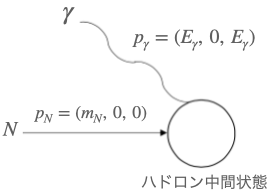
\includegraphics[height=5cm]{img/diagram_momentum.png}
    \caption{ハドロン中間状態と核子と光子の図}
    \label{fig:sigma1}
\end{figure}

\subsection{宇宙線$\mu$の仮定}
宇宙線$\mu$ のエネルギー$E_\mu$ は$E_\gamma$ よりも遥かに大きいエネルギーを持つ必要がある。
そのため$E_\mu = 1.5$ GeV とおく。
また$E_\mu = 1.5$ GeV 以上となる$\mu$ の割合Rは\ref{fig:sigma2}より$R \approx 0.56$ と頻度が高めである。


\begin{figure}[H]
    \centering
    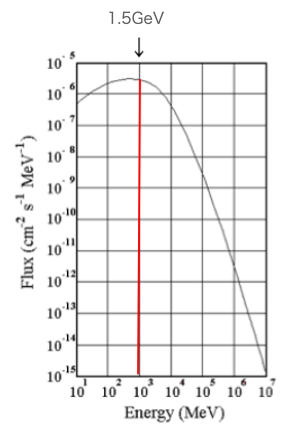
\includegraphics[height=5cm]{img/cosimic_ray_energy_distribution.png}
    \caption{宇宙線$\mu$のエネルギー分布 \cite{myThesisTest1}}
    \label{fig:sigma2}
\end{figure}

$E_\mu$と散乱後の$\mu$のエネルギー$E'_\mu$ との比をyとして、その値は
\begin{equation}
    y = \dfrac{E_\mu - E'_\mu}{E_\mu} \approx 0.2
\end{equation}

\section{生成断面積の計算枠組み}
$\mu$とNの散乱断面積$\sigma_{\mu N}$は$\mu$から$\gamma$を出す確率$\Phi$と、
$\gamma$とNとの散乱断面積$\sigma_{tot}(\gamma^* N)$の積で表すことができる。

\begin{equation}
    \sigma_{\mu N} =\int dy  \sigma_{tot}(\gamma^* N) \Phi(y)
\end{equation}

また、$\Phi(y)$は以下のように表す。
\begin{equation}
    \Phi(y) = \dfrac{\alpha}{\pi y} \int \dfrac{dQ^2}{Q^2} [(1-y)(1 - \dfrac{Q^2_{min}}{Q^2}) + \dfrac{y^2}{2}]
\end{equation}

$Q^2$を運動量移行の2乗の負数とした。


\section{\texorpdfstring{$\Phi$}{LG}の考察}
$\Phi$の積分前の関数はyを定数とすることで\ref{fig:sigma3}のようになる。
\begin{figure}[H]
    \centering
    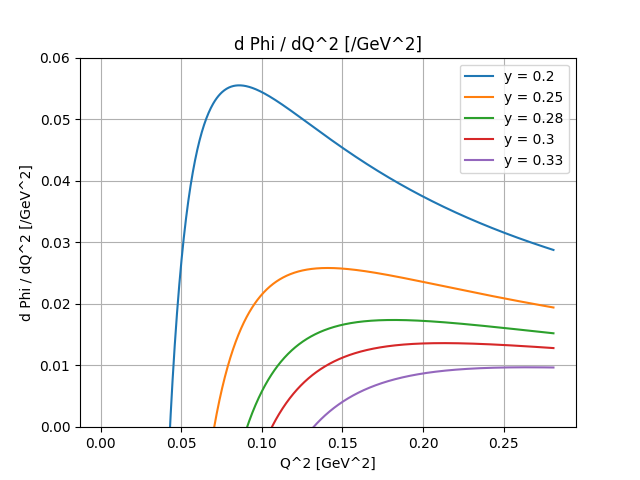
\includegraphics[height=5cm]{img/flux_fixed_y.png}
    \caption{$\dfrac{d\Phi ^2}{dydQ^2}$ のyを定数としたグラフ}
    \label{fig:sigma3}
\end{figure}

このグラフから$\Phi$はyが小さいところで大きくなる。つまり、$E_\mu$ が $E_\gamma$より遥かに大きくなるところで$\sigma_{\mu N}$が大きくなる。
また、$Q^2$が小さくなるところで大きくなっている。$Q^2$は0でない最小値を持つ。


\section{断面積の計算に用いる近似}
$E_\gamma = [300, 500]$MeVと仮定する。
\ref{fig:sigma4}を用いて$\gamma$とNの反応断面積$\sigma_{tot}(\gamma^* N)$を
$\sigma_{tot}(\gamma^* N) = 0.3$ mbと近似する。
\begin{figure}[H]
    \centering
    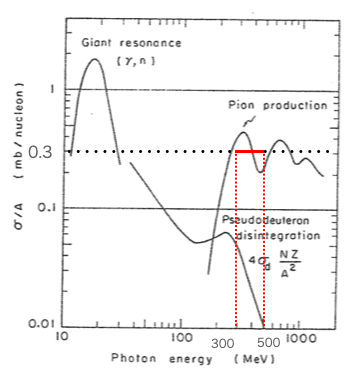
\includegraphics[height=5cm]{img/sigma_tot.png}
    \caption{核子1個あたりの全光核反応断面積と光子のエネルギーの関係}
    \label{fig:sigma4}
\end{figure}

$E_\mu = 1.5$GeV,$E_\gamma = [0.3, 0.5]$GeVの仮定からyの範囲は
\begin{equation}
    y = \dfrac{E_\gamma}{E_\mu}
\end{equation}
を用いることで$y = [0.20, 0.33]$となる。


\section{積分範囲}
$m_W$の関係式$m_W = \sqrt{m_p^2 + 2m_pE_\mu y - Q^2}$は
$m_W = 1.08$GeVとした時、\ref{fig:sigma5}のようになる。

\begin{figure}[H]
    \centering
    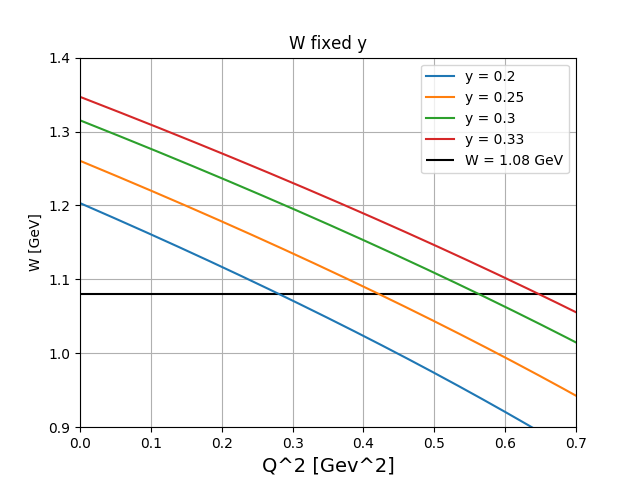
\includegraphics[height=5cm]{img/W2_fixed_y.png}
    \caption{$m_W = \sqrt{m_p^2 + 2m_pE_\mu y - Q^2}$のyを固定した関係式}
    \label{fig:sigma5}
\end{figure}

$m_W = 1.08$GeVの直線とyの値ごとの直線が交わる$Q^2$の値が$Q^2$の最大値になりこの$Q^2$を$Q^2_{max}$とする。

よって、積分範囲は$y = [0.20, 0.33], Q^2 = [Q^2_{min}(y), Q^2_{max}(y)]$となる。

\section{断面積の計算}
$\dfrac{d^2\sigma}{dydQ^2}$は\ref{fig:sigma6}のようになる。

\begin{figure}[H]
    \centering
    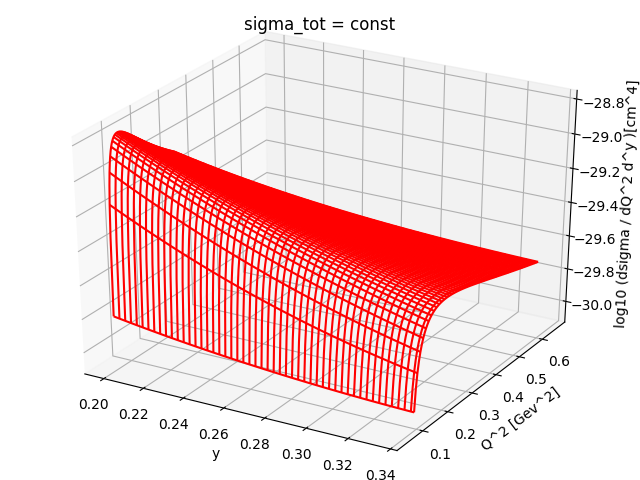
\includegraphics[width=8cm]{img/integrate_flux_used_artile.png}
    \caption{$\dfrac{d^2\sigma}{dydQ^2}$の3次元プロット}
    \label{fig:sigma6}
\end{figure}

これを積分すると、$\sigma \approx 3.3 \times 10^{-28} cm^2$となった。

\section{予定する検出器でのイベント数の見積もり}
関係式
\begin{equation}
    -dN =\dfrac{\rho N_A \sigma }{A}NRV
\end{equation}
から反応式を見積もる。

$-dN$を入射$\mu$の単位時間あたりの減少分、検出器の密度$\rho = 1.0 g/cm^2$、
検出器の質量数$A = 12 g/mol$、検出器の有効体積$V = 7500cm^3$、
単位時間・単位面積あたりの入射する$\mu$の数を$N = \dfrac{1}{10\times 10} 個/s\cdot cm^2$、
1.5GeV以上のエネルギーを持ち$\mu$の割合を$R = 0.56$として代入すると
\begin{equation}
    -dN \approx 4.4 \times 10^{-4}(個/s)
\end{equation}
となった。